% Copyright 2019 by Till Tantau
%
% This file may be distributed and/or modified
%
% 1. under the LaTeX Project Public License and/or
% 2. under the GNU Free Documentation License.
%
% See the file doc/generic/pgf/licenses/LICENSE for more details.

 
\section{Design Principles\\设计原则}

This section describes the design principles behind the \tikzname\ frontend,
where \tikzname\ means ``\tikzname\ ist \emph{kein} Zeichenprogramm''. To use
\tikzname, as a \LaTeX\ user say |\usepackage{tikz}| somewhere in the preamble,
as a plain \TeX\ user say |\input tikz.tex|. \tikzname's job is to make your
life easier by providing an easy-to-learn and easy-to-use syntax for describing
graphics.

本节介绍了\tikzname\ 前端的设计原则,其中\tikzname\ 表示``\tikzname\ 不是绘图软件''。要使用\tikzname,作为\LaTeX\ 用户,在导言区中的某处使用|\usepackage{tikz}|;作为plain \TeX\ 用户,在导言区中使用|\input tikz.tex|。通过提供易于学习和使用的语法来描述图形,\tikzname\ 的任务是使您的生活更加轻松。

The commands and syntax of \tikzname\ were influenced by several sources. The
basic command names and the notion of path operations is taken from
\textsc{metafont}, the option mechanism comes from \textsc{pstricks}, the
notion of styles is reminiscent of \textsc{svg}, the graph syntax is taken from
\textsc{graphviz}. To make it all work together, some compromises were
necessary. I also added some ideas of my own, like coordinate transformations.

\tikzname\ 的命令和语法受到多种来源的影响。基本命令名称和路径操作的概念来自\textsc{metafont},选项机制来自\textsc{pstricks},样式的概念类似于\textsc{svg},图形语法来自\textsc{graphviz}。为了使所有这些工作协同工作,进行了一些妥协。我还添加了一些我自己的想法,比如坐标转换。


The following basic design principles underlie \tikzname:

以下是\tikzname\ 的基本设计原则:
%
\begin{enumerate}
    \item Special syntax for specifying points.

    用于指定点的特殊语法。
    \item Special syntax for path specifications.

    用于路径规范的特殊语法。
    \item Actions on paths.

    路径上的操作。
    \item Key--value syntax for graphic parameters.

    图形参数的键-值语法。
    \item Special syntax for nodes.

    节点的特殊语法。
    \item Special syntax for trees.

    树的特殊语法。
    \item Special syntax for graphs.

    

    图的特殊语法。
    \item Grouping of graphic parameters.

    图形参数的分组。
    \item Coordinate transformation system.

    坐标转换系统。
\end{enumerate}



\subsection{Special Syntax For Specifying Points\\用于指定点的特殊语法}

\tikzname\ provides a special syntax for specifying points and coordinates. In
the simplest case, you provide two \TeX\ dimensions, separated by commas, in
round brackets as in |(1cm,2pt)|.

\tikzname\ 提供了一种特殊的语法来指定点和坐标。在最简单的情况下,您可以在圆括号中用逗号分隔的两个\TeX\ 尺寸来指定点,如|(1cm,2pt)|。

You can also specify a point in polar coordinates by using a colon instead of a
comma as in |(30:1cm)|, which means ``1cm in a 30 degrees direction''.

您还可以使用冒号而不是逗号来指定点的极坐标,如|(30:1cm)|,表示``在30度方向上1cm''。

If you do not provide a unit, as in |(2,1)|, you specify a point in \pgfname's
$xy$-coordinate system. By default, the unit $x$-vector goes 1cm to the right
and the unit $y$-vector goes 1cm upward.

如果您没有提供单位,比如|(2,1)|,则指定了\pgfname 的$xy$坐标系中的一个点。默认情况下,单位$x$向量向右移动1cm,单位$y$向量向上移动1cm。

By specifying three numbers as in |(1,1,1)| you specify a point in \pgfname's
$xyz$-coordinate system.

通过指定三个数字,如|(1,1,1)|,您可以指定\pgfname 的$xyz$坐标系中的一个点。

It is also possible to use an anchor of a previously defined shape as in
|(first node.south)|.

也可以使用先前定义的形状的锚点,如|(first node.south)|。

You can add two plus signs before a coordinate as in |++(1cm,0pt)|. This means
``1cm to the right of the last point used''. This allows you to easily specify
relative movements. For example, |(1,0) ++(1,0) ++(0,1)| specifies the three
coordinates |(1,0)|, then |(2,0)|, and |(2,1)|.

您可以在坐标之前加上两个加号,如|++(1cm,0pt)|。这表示``在上次使用的点的右侧1cm''。这使您可以轻松地指定相对移动。例如,|(1,0) ++(1,0) ++(0,1)| 指定了三个坐标|(1,0)|,然后是|(2,0)|,最后是|(2,1)|。

Finally, instead of two plus signs, you can also add a single one. This also
specifies a point in a relative manner, but it does not ``change'' the current
point used in subsequent relative commands. For example, |(1,0) +(1,0) +(0,1)|
specifies the three coordinates |(1,0)|, then |(2,0)|, and |(1,1)|.

最后,您还可以添加一个加号。这也以相对方式指定一个点,但它不会``更改''后续相对命令中使用的当前点。例如,|(1,0) +(1,0) +(0,1)| 指定了三个坐标|(1,0)|,然后是|(2,0)|,最后是|(1,1)|。


\subsection{Special Syntax For Path Specifications\\用于路径规范的特殊语法}

When creating a picture using \tikzname, your main job is the specification of
\emph{paths}. A path is a series of straight or curved lines, which need not be
connected. \tikzname\ makes it easy to specify paths, partly using the syntax
of \textsc{metapost}. For example, to specify a triangular path you use

使用\tikzname\ 创建图时,您的主要工作是指定\emph{路径}。路径是一系列直线或曲线,不一定相连。通过部分使用\textsc{metapost}的语法,\tikzname\ 使得指定路径变得容易。例如,要指定一个三角形路径,可以使用以下语法:
%
\begin{codeexample}[code only]
(5pt,0pt) -- (0pt,0pt) -- (0pt,5pt) -- cycle
\end{codeexample}
%
and you get \tikz \draw (5pt,0pt) -- (0pt,0pt) -- (0pt,5pt) -- cycle; when you
draw this path.

当你绘制该路径时,你会得到\tikz \draw (5pt,0pt) -- (0pt,0pt) -- (0pt,5pt) -- cycle;。


\subsection{Actions on Paths\\路径操作}

A path is just a series of straight and curved lines, but it is not yet
specified what should happen with it. One can \emph{draw} a path, \emph{fill} a
path, \emph{shade} it, \emph{clip} it, or do any combination of these. Drawing
(also known as \emph{stroking}) can be thought of as taking a pen of a certain
thickness and moving it along the path, thereby drawing on the canvas. Filling
means that the interior of the path is filled with a uniform color. Obviously,
filling makes sense only for \emph{closed} paths and a path is automatically
closed prior to filling, if necessary.

路径只是一系列直线和曲线,但尚未指定应该对其执行什么操作。可以对路径进行\emph{绘制}、\emph{填充}、\emph{渐变}、\emph{裁剪}或进行这些操作的任意组合。绘制(也称为\emph{描边})可以看作是沿着路径移动一支特定粗细的笔,从而在画布上绘制图形。填充意味着用均匀的颜色填充路径的内部。显然,填充只适用于\emph{闭合}路径,并且如果需要,路径会在填充之前自动闭合。


Given a path as in |\path (0,0) rectangle (2ex,1ex);|, you can draw it by
adding the |draw| option as in |\path[draw] (0,0) rectangle (2ex,1ex);|, which
yields \tikz \path[draw] (0,0) rectangle (2ex,1ex);. The |\draw| command is
just an abbreviation for |\path[draw]|. To fill a path, use the |fill| option
or the |\fill| command, which is an abbreviation for |\path[fill]|. The
|\filldraw| command is an abbreviation for |\path[fill,draw]|. Shading is
caused by the |shade| option (there are |\shade| and |\shadedraw|
abbreviations) and clipping by the |clip| option. There is also a |\clip|
command, which does the same as |\path[clip]|, but not commands like
|\drawclip|. Use, say, |\draw[clip]| or |\path[draw,clip]| instead.

给定路径 |\path (0,0) rectangle (2ex,1ex);|,你可以通过添加 |draw| 选项来绘制它,如\\|\path[draw] (0,0) rectangle (2ex,1ex);|,结果为 \tikz \path[draw] (0,0) rectangle (2ex,1ex);。|\draw| 命令只是 |\path[draw]| 的缩写。要填充路径,请使用 |fill| 选项或 |\fill| 命令,它是 |\path[fill]| 的缩写。|\filldraw| 命令是 |\path[fill,draw]| 的缩写。通过 |shade| 选项(有 |\shade| 和 |\shadedraw| 的缩写)可以产生渐变效果,通过 |clip| 选项进行裁剪。还有一个 |\clip| 命令,它与 |\path[clip]| 相同,但没有像 |\drawclip| 这样的命令。代替使用 |\drawclip|,可以使用 |\draw[clip]| 或 |\path[draw,clip]|。

All of these commands can only be used inside |{tikzpicture}| environments.

所有这些命令只能在 |{tikzpicture}| 环境中使用。

\tikzname\ allows you to use different colors for filling and stroking.

\tikzname\ 允许你使用不同的颜色进行填充和描边。


\subsection{Key--Value Syntax for Graphic Parameters\\图形参数的键-值语法}

Whenever \tikzname\ draws or fills a path, a large number of graphic parameters
influences the rendering. Examples include the colors used, the dashing
pattern, the clipping area, the line width, and many others. In \tikzname, all
these options are specified as lists of so called key--value pairs, as in
|color=red|, that are passed as optional parameters to the path drawing and
filling commands. This usage is similar to \textsc{pstricks}. For example, the
following will draw a thick, red triangle;

每当\tikzname\ 绘制或填充路径时,许多图形参数会影响渲染结果。例如,使用的颜色、虚线模式、裁剪区域、线宽等等。在\tikzname\ 中,所有这些选项都被指定为所谓的键-值对列表,比如 |color=red|,作为可选参数传递给路径绘制和填充命令。这种用法类似于 \textsc{pstricks}。例如,下面的代码将绘制一个粗红色的三角形:
%
\begin{codeexample}[]
\tikz \draw[line width=2pt,color=red] (1,0) -- (0,0) -- (0,1) -- cycle;
\end{codeexample}


\subsection{Special Syntax for Specifying Nodes\\指定节点的特殊语法}

\tikzname\ introduces a special syntax for adding text or, more generally,
nodes to a graphic. When you specify a path, add nodes as in the following
example:

\tikzname\ 引入了一种特殊的语法,用于向图形添加文本或更一般的节点。当你指定一个路径时,可以像以下示例中那样添加节点:
%
\begin{codeexample}[]
\tikz \draw (1,1) node {text} -- (2,2);
\end{codeexample}
%
Nodes are inserted at the current position of the path, but either \emph{after}
(the default) or \emph{before} the complete path is rendered. When special
options are given, as in |\draw (1,1) node[circle,draw] {text};|, the text is
not just put at the current position. Rather, it is surrounded by a circle and
this circle is ``drawn''.

节点被插入到路径的当前位置,但在完整路径渲染之前,要么\emph{之后}(默认),要么\emph{之前}。当给定特殊选项时,比如 |\draw (1,1) node[circle,draw] {text};|,文本不仅仅放在当前位置上,而是被一个圆圈包围,并且这个圆圈被“绘制”。

You can add a name to a node for later reference either by using the option
|name=|\meta{node name} or by stating the node name in parentheses outside the
text as in |node[circle](name){text}|.

% 你可以通过使用选项|name=|\meta{节点名称}或在文本之外的括号中指定节点名称,为节点添加名称以供以后引用。
你可以通过使用选项 |name=|\meta{节点名称} 或者在文本外部的括号中指定节点名称,来为节点添加名称以供以后引用,例如 |node[circle](name){text}|.。



Predefined shapes include |rectangle|, |circle|, and |ellipse|, but it is
possible (though a bit challenging) to define new shapes.

预定义的形状包括|rectangle|、|circle|和|ellipse|,但也可以(尽管有点困难)定义新的形状。


\subsection{Special Syntax for Specifying Trees\\树结构的特殊语法}

The ``node syntax'' can also be used to draw tress: A |node| can be followed by
any number of children, each introduced by the keyword |child|. The children
are nodes themselves, each of which may have children in turn.

“节点语法”也可用于绘制树结构:一个|node|后面可以跟随任意数量的子节点,每个子节点都以关键字|child|引入。子节点本身也可以有子节点。


%
\begin{codeexample}[]
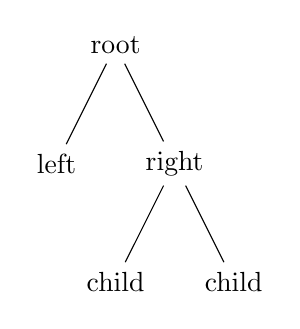
\begin{tikzpicture}
  \node {root}
    child {node {left}}
    child {node {right}
      child {node {child}}
      child {node {child}}
    };
\end{tikzpicture}
\end{codeexample}
%
Since trees are made up from nodes, it is possible to use options to modify the
way trees are drawn. Here are two examples of the above tree, redrawn with
different options:

由于树结构由节点构成,可以使用选项修改绘制树结构的方式。以下是上述树结构的两个示例,使用不同的选项重新绘制:


%
\begin{codeexample}[preamble={\usetikzlibrary{arrows.meta,trees}}]
\begin{tikzpicture}
  [edge from parent fork down, sibling distance=15mm, level distance=15mm,
   every node/.style={fill=red!30,rounded corners},
   edge from parent/.style={red,-{Circle[open]},thick,draw}]
  \node {root}
      child {node {left}}
      child {node {right}
        child {node {child}}
        child {node {child}}
      };
\end{tikzpicture}
\end{codeexample}

\begin{codeexample}[]
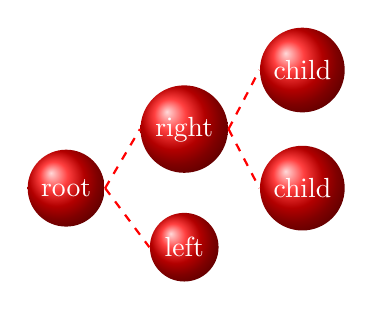
\begin{tikzpicture}
  [parent anchor=east,child anchor=west,grow=east,
   sibling distance=15mm, level distance=15mm,
   every node/.style={ball color=red,circle,text=white},
   edge from parent/.style={draw,dashed,thick,red}]
  \node {root}
      child {node {left}}
      child {node {right}
        child {node {child}}
        child {node {child}}
      };
\end{tikzpicture}
\end{codeexample}


\subsection{Special Syntax for Graphs\\图结构的特殊语法}

The |\node| command gives you fine control over where nodes should be placed,
what text they should use, and what they should look like. However, when you
draw a graph, you typically need to create numerous fairly similar nodes that
only differ with respect to the name they show. In these cases, the |graph|
syntax can be used, which is another syntax layer build ``on top'' of the node
syntax.

|\node|命令使您可以精确控制节点的位置、文本和外观。然而,在绘制图结构时,通常需要创建许多具有相似特征但在显示名称方面略有不同的节点。在这些情况下,可以使用|graph|语法,它是在节点语法之上构建的另一种语法层。

%
\begin{codeexample}[preamble={\usetikzlibrary{graphs}}]
\tikz \graph [grow down, branch right] {
  root -> { left, right -> {child, child} }
};
\end{codeexample}
%
The syntax of the |graph| command extends the so-called \textsc{dot}-notation
used in the popular \textsc{graphviz} program.

|graph|命令的语法扩展了流行的\textsc{graphviz}程序中使用的所谓\textsc{dot}表示法。

Depending on the version of \TeX\ you use (it must allow you to call Lua code,
which is the case for Lua\TeX), you can also ask \tikzname\ to do automatically
compute good positions for the nodes of a graph using one of several integrated
\emph{graph drawing algorithms}.

根据您使用的\TeX{}版本(它必须允许调用Lua代码,这适用于Lua\TeX),您还可以请求\tikzname{}使用多个集成的\emph{图绘制算法}自动计算图的节点的良好位置。


\subsection{Grouping of Graphic Parameters\\图形参数的分组}

Graphic parameters should often apply to several path drawing or filling
commands. For example, we may wish to draw numerous lines all with the same
line width of 1pt. For this, we put these commands in a |{scope}| environment
that takes the desired graphic options as an optional parameter. Naturally, the
specified graphic parameters apply only to the drawing and filling commands
inside the environment. Furthermore, nested |{scope}| environments or
individual drawing commands can override the graphic parameters of outer
|{scope}| environments. In the following example, three red lines, two green
lines, and one blue line are drawn:

图形参数通常应用于多个路径绘制或填充命令。例如,我们可能希望绘制许多具有相同线宽(1pt)的线条。为此,我们将这些命令放在|{scope}|环境中,并将所需的图形选项作为可选参数传递。显然,指定的图形参数仅适用于环境内部的绘制和填充命令。此外,嵌套的|{scope}|环境或单独的绘制命令可以覆盖外部|{scope}|环境的图形参数。在下面的示例中,绘制了三条红线、两条绿线和一条蓝线:

%
\begin{codeexample}[]
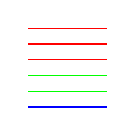
\begin{tikzpicture}
  \begin{scope}[color=red]
    \draw (0mm,10mm) -- (10mm,10mm);
    \draw (0mm, 8mm) -- (10mm, 8mm);
    \draw (0mm, 6mm) -- (10mm, 6mm);
  \end{scope}
  \begin{scope}[color=green]
    \draw             (0mm, 4mm) -- (10mm, 4mm);
    \draw             (0mm, 2mm) -- (10mm, 2mm);
    \draw[color=blue] (0mm, 0mm) -- (10mm, 0mm);
  \end{scope}
\end{tikzpicture}
\end{codeexample}

The |{tikzpicture}| environment itself also behaves like a |{scope}|
environment, that is, you can specify graphic parameters using an optional
argument. These optional apply to all commands in the picture.

|{tikzpicture}|环境本身也像|{scope}|环境一样,可以使用可选参数指定图形参数。这些可选参数适用于图中的所有命令。


\subsection{Coordinate Transformation System\\坐标变换系统}

\tikzname\ supports both \pgfname's \emph{coordinate} transformation system to
perform transformations as well as \emph{canvas} transformations, a more
low-level transformation system. (For details on the difference between
coordinate transformations and canvas transformations see
Section~\ref{section-design-transformations}.)


\tikzname{}支持\pgfname{}的\emph{坐标变换}系统和更底层的\emph{画布变换}系统两种转换方式。 (有关坐标变换和画布变换之间差异的详细信息,请参见第\ref{section-design-transformations}节。)

The syntax is set up in such a way that it is harder to use canvas
transformations than coordinate transformations. There are two reasons for
this: First, the canvas transformation must be used with great care and often
results in ``bad'' graphics with changing line width and text in wrong sizes.
Second, \pgfname\ loses track of where nodes and shapes are positioned when
canvas transformations are used. So, in almost all circumstances, you should
use coordinate transformations rather than canvas transformations.

语法设置得更难使用画布变换而不是坐标变换。这有两个原因:首先,必须非常小心地使用画布变换,否则往往会得到“糟糕”的图形,包括线宽变化和文本大小错误的情况。其次,在使用画布变换时,\pgfname{}无法追踪节点和形状的位置。因此,在几乎所有情况下,应该使用坐标变换而不是画布变换。

